% !TEX root = ../main.tex
%
\chapter{Application Design}
\label{sec:design}

\section{Design Process}
\label{sec:design:ux}

The transition from the initial findings of user research to the creation of a functional prototype was a multi-step process focused on the capture of user needs and their translation into a tangible design.
This section outlines the process of transforming abstract requirements into a functional prototype, with particular emphasis on the methodologies employed at each stage of the process.

\subsection*{From User Research to User Flow Diagram}

Following the completion of initial user research, the first step involved modeling the key findings into a user flow diagram (Figure \ref{fig:design:flow-1}).
This diagram served as a visual representation of the user's journey through the prototype, highlighting the key interactions users would have with the system.

\begin{figure}[h!]
	\includegraphics[width=\textwidth]{figures/flow-1.png}
	\caption{User flow diagram illustrating the key interactions for creating a NeRF model}
	\label{fig:design:flow-1}
\end{figure}

The objective of the user flow diagram was twofold: firstly, to map out the envisioned user experience, and secondly, to identify any potential bottlenecks or usability issues at an early stage of the design process.

\subsection*{Developing the Site Map}

Building upon the foundation established by the user flow diagram, the next stage involved the expansion of this outline into a detailed site map.
The site map offered a more comprehensive view of the prototype's structure, delineating the relationships between different pages and features.
This excerpt from the site map (Figure \ref{fig:design:flow-2}) illustrates the level of detail and complexity involved in mapping out the prototype's user interactions.

\begin{figure}[htb]
  \centering
  \includegraphics[width=.8\textwidth]{figures/flow-2.png}
  \caption{Excerpt of a view from the flow diagram with detailed interactions.}
  \label{fig:design:flow-2}
\end{figure}

This expanded view was instrumental in ensuring that the user flow remained structured across the broader system, facilitating easy navigation and a cohesive user experience.

\subsection*{Wireframing}

With a firm grasp on the user flow and site structure, the focus shifted to wireframing. The initial wireframes were created to model the overall layout of the interface, providing a skeletal framework for the visual design. These wireframes were intentionally kept simple to prioritize structural and functional decisions over aesthetic considerations \fref{fig:design:wireframe}.
At this stage, emphasis was placed on the placement of key elements, usability, and adherence to the user flow and site map.

\begin{figure}[h!]
  \centering
  \includegraphics[width=.8\textwidth]{figures/wireframe.png}
  \caption{Wireframe of the pre-processing section, showing the layout and key elements.}
  \label{fig:design:wireframe}
\end{figure}

\subsection*{Refinement Through Development}

The transition from wireframes to a functioning prototype was achieved through a process of iterative refinement during the development phase.
As the prototype developed, the initial designs were subjected to continuous evaluation and adjustment based on practical considerations and technical constraints.
This phase permitted a deeper exploration of interactions, animations, and the overall look and feel of the interface.
During this period, the wireframes underwent a transformation into a more detailed and user-friendly interface, with adjustments made as necessary to enhance usability and ensure a seamless user experience.

\section{User Interface Design}
The user interface was designed to be as simple as possible while still providing all necessary functionality.
The design of the prototype can be divided into two primary sections: a dashboard that provides an overview of all projects and a project section that provides users with the necessary tools to create and edit NeRF models.

\subsection*{Dashboard}

The dashboard is the initial view that users encounter when launching the application.
It displays all previously created projects and enables users to create new ones.
Each project is represented as a card, which includes the project name, a preview of the provided input images (if present), and tags that indicate the current status of the project \frefadd{fig:design:dashboard}{1}.
Additionally, a separate card is available through which users can create a new project by providing a name \frefadd{fig:design:dashboard}{2}.
To open a project, one must simply click on the respective card.
When creating a new project, users are redirected to the project section.

\begin{figure}[htb]
  \centering
  \includegraphics[width=.65\textwidth]{figures/view-overview.png}
  \caption{Dashboard overview, showing existing projects (1) and the option to create a new project (2).}
  \label{fig:design:dashboard}
\end{figure}

\subsection*{Project Section}

The project section represents the core of the application, through which users can create and edit NeRF models.
The section is divided into three distinct sections: the input section, the training section, and the rendering section.
In all sections, users can monitor their progress through a progress indicator located at the top of the screen, which also facilitates straightforward navigation between the various sections \frefadd{fig:design:input-section}{1}.

\subsubsection*{Input Section}

The input section combines the first few interactions, as mapped out in the user flow diagram.
Initially, users are prompted to upload their input data, which can be done by either dragging and dropping files into the browser window or by clicking a button to open a file dialog \frefadd{fig:design:input-section}{2}.
Files may be either a set of images, a video or archives used for Polycam or Record3D.
To ensure the input data is valid, certain guardrails are in place, such as file type restrictions.
Once the input data has been uploaded, it must be processed before it can be used for training purposes.

\begin{figure}[h!]
  \centering
  \includegraphics[width=.65\textwidth]{figures/view-process.png}
  \caption{Pre-processing section, showing the progress bar (1), input data upload (2), parameter options (3), pre-processed data list (4), and console output (5).}
  \label{fig:design:input-section}
\end{figure}

The pre-processing can be configured by the user, which includes parameters such as the lens type or matching method \frefadd{fig:design:input-section}{3}.
The parameter input fields vary based on the type of input data and are only shown when relevant. 
Additionally, a tooltip is provided for each parameter, explaining its purpose. 
Furthermore, advanced settings can be accessed by hovering over the question mark next to the parameter name.
For advanced users, the settings can be further customized by activating the advanced settings using the toggle in the top right \fref{fig:design:advanced-settings}.
Once the user is satisfied with the settings, they can initiate the pre-processing. The user will then be able to observe the progress of the pre-processing through a console that displays the output of the process running on the server \frefadd{fig:design:input-section}{5}.
Upon completion of the pre-processing stage, the user may then proceed to the training section.

\begin{figure}[h!]
  \centering
  \includegraphics[width=.65\textwidth]{figures/view-extended-options.png}
  \caption{Advanced settings for pre-processing, showing additional parameters and options.}
  \label{fig:design:advanced-settings}
\end{figure}

In case the data was already pre-processed, a list is visible that shows all available pre-processed data, and the user can select one to use for training \frefadd{fig:design:input-section}{4}.
Users can also inspect the configuration with which the data was pre-processed, and delete it if necessary.

\subsubsection*{Training Section}

The training section is structured similarly to the input section, with a form that allows users to configure the training process \frefadd{fig:design:training-section}{1}, and a console that displays the output of the training process running on the server.
Once the user is satisfied with the configuration, they can start the training process.

\begin{figure}[h!]
  \centering
  \includegraphics[width=.65\textwidth]{figures/view-train.png}
  \caption{Training section, showing the training configuration form (1), and previous training runs (2).}
  \label{fig:design:training-section}
\end{figure}

Previous training runs are listed, and users can inspect the configuration with which the training was run, and delete it if necessary \frefadd{fig:design:input-section}{2}.
The viewer can be opened to inspect the results of the training run, or an existing checkpoint can be selected to resume training from that point.

\subsubsection*{Viewer Section}

The final step in the process is the viewer section, which allows users to inspect their NeRF model while it is still training or after the training has finished \frefadd{fig:design:viewer-section}{1}.
At its core is the Nerfstudio Viewer, which is integrated into the application.
The integrated version provides users with all the functionality available in the standalone version, with a few integrations that simplify the rendering process.
Instead of providing commands that have to be executed in the terminal, the rendering is started by clicking a button.
The renders are listed below the viewer, and once they finish processing, they can be downloaded to the user's machine \frefadd{fig:design:viewer-section}{2}.
Due to the narrow layout of the page, the viewer can be conveniently opened in a new tab to provide a better viewing experience.

\begin{figure}[h!]
  \centering
  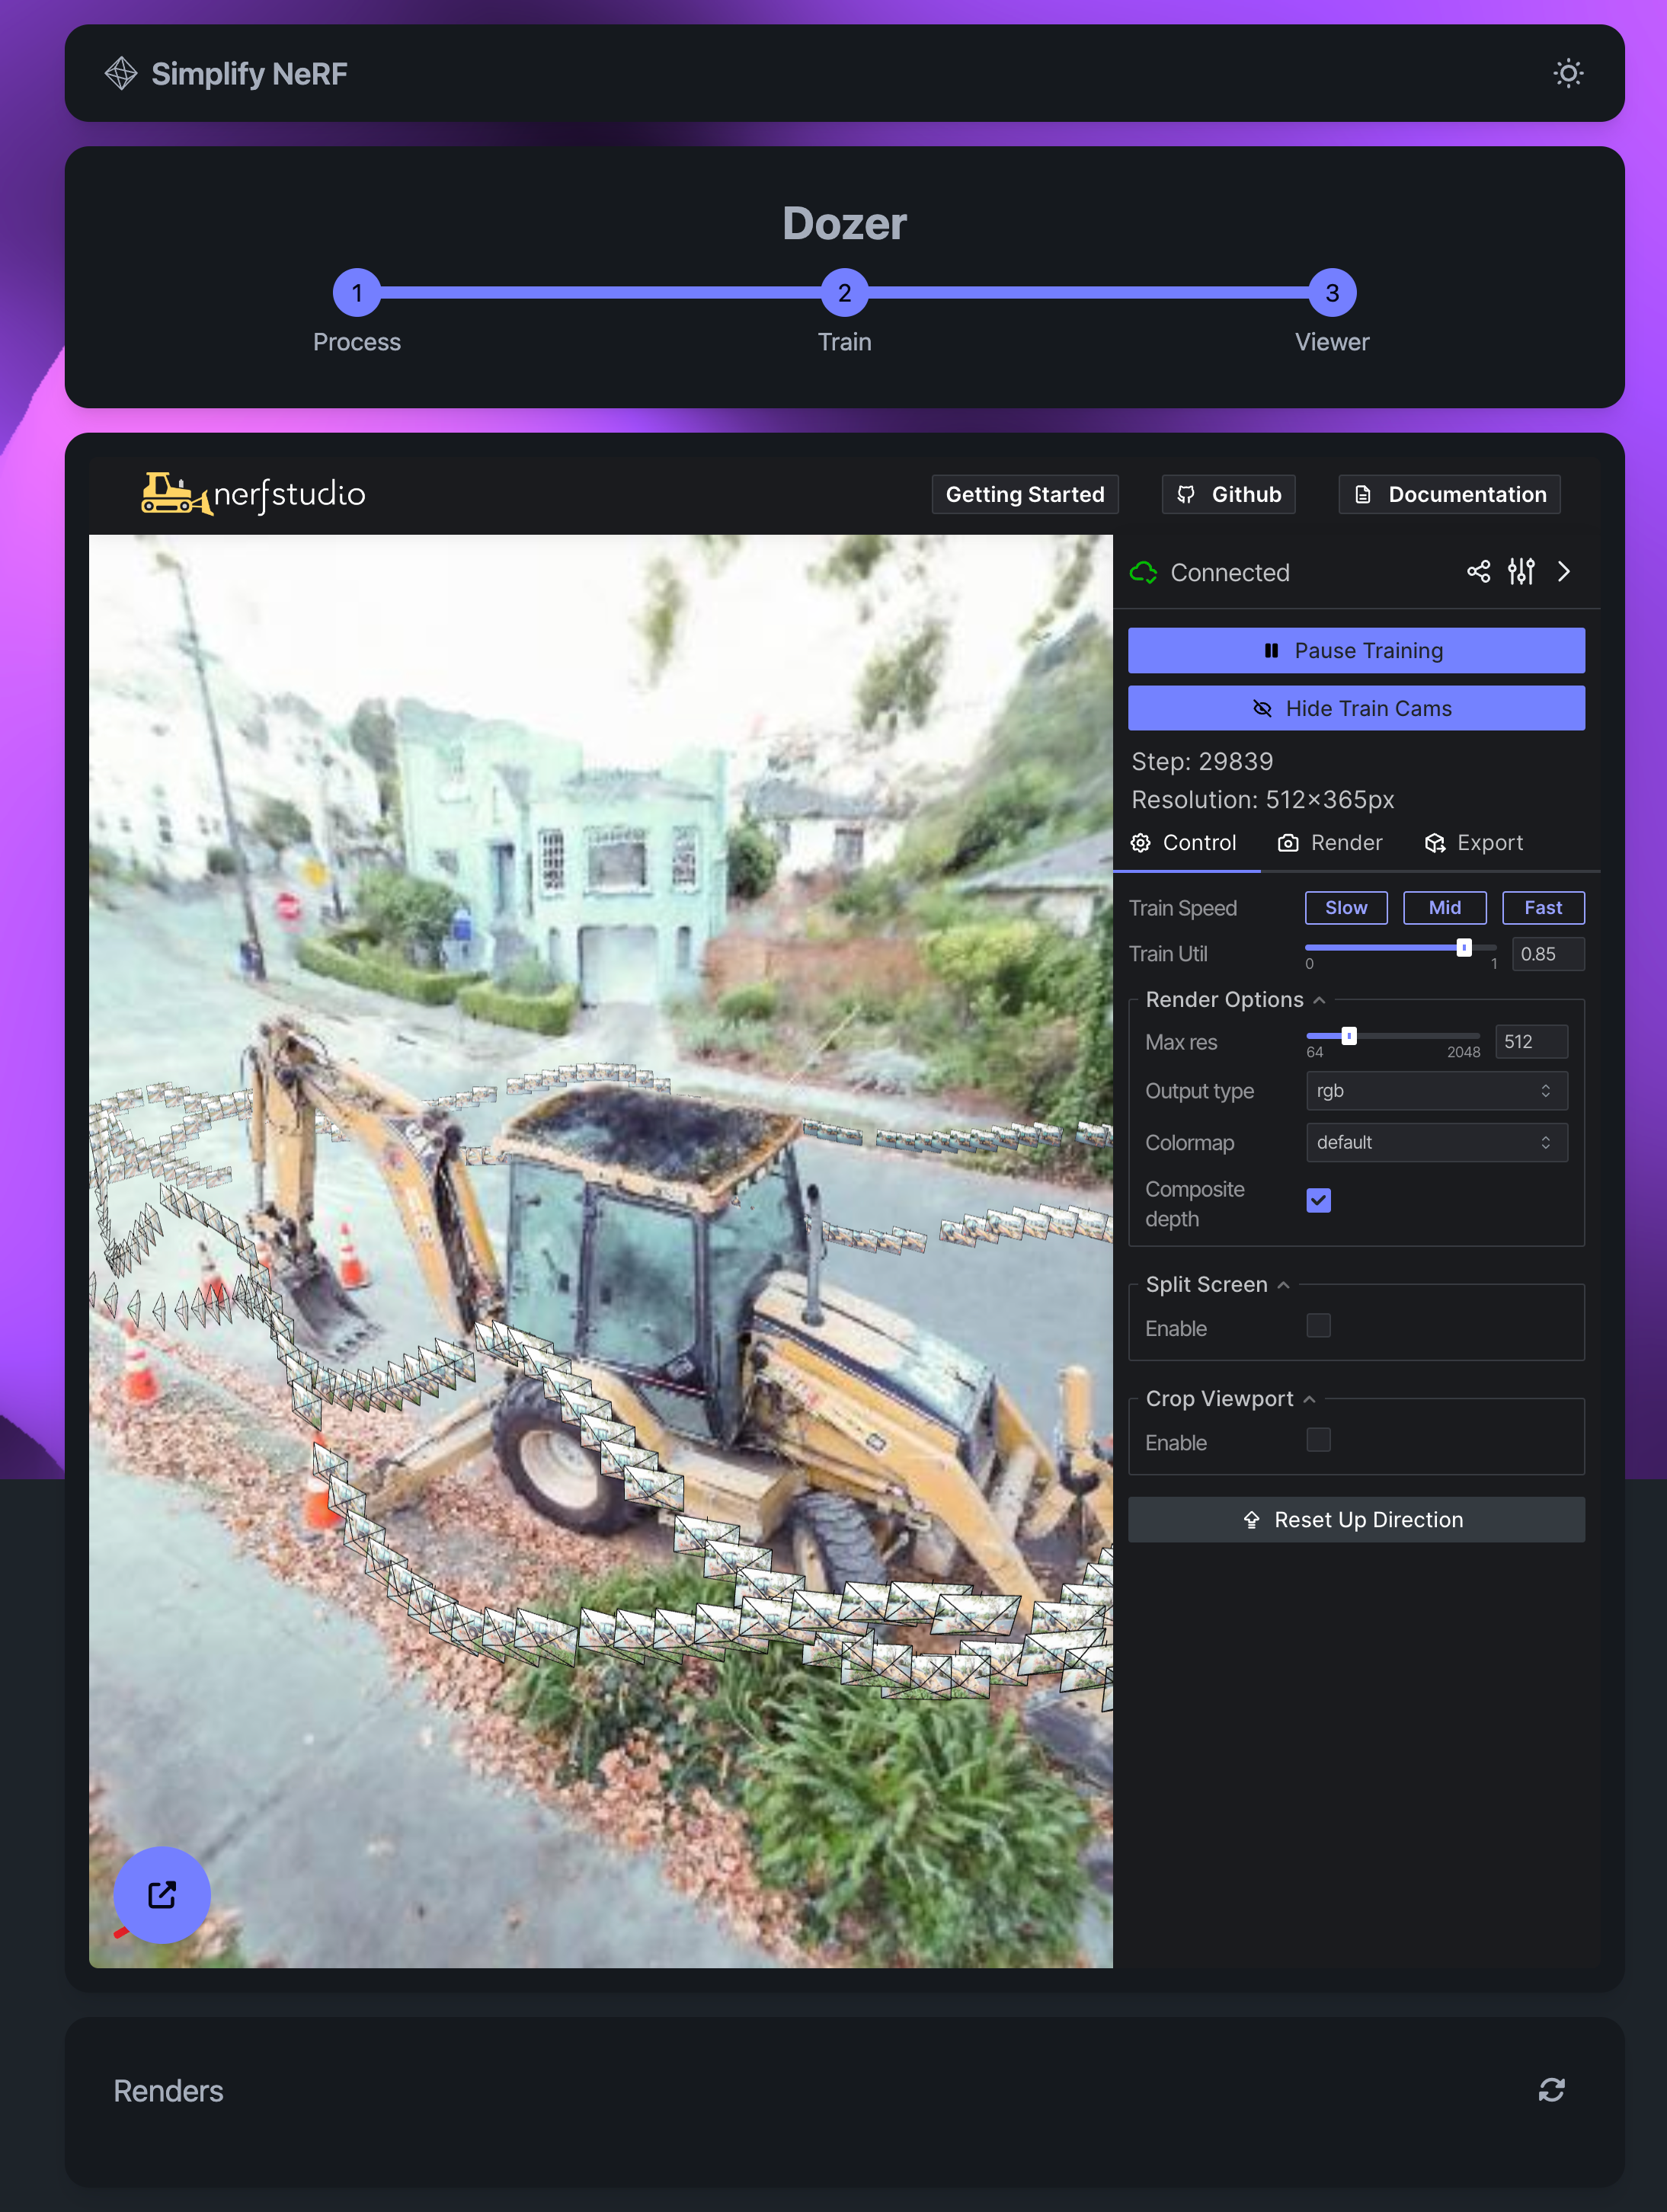
\includegraphics[width=.65\textwidth]{figures/view-viewer.png}
  \caption{Viewer section, showing the Nerfstudio viewer (1) and list of rendered outputs (2).}
  \label{fig:design:viewer-section}
\end{figure}
